%% content.tex
%%

%% ==============
\chapter{Content Chapters}
\label{ch:Content1}
%% ==============

% The content chapters of your thesis should of course be renamed. How many chapters you need to write depends on your thesis and cannot be said in general.

%  Always reference figures, tables etc. To give a few simple examples, this section contains Algorithm \ref{theorem:doof}, Table \ref{tbl:randomnumbers}, Figure \ref{fig:somegraph}, and Theorem \ref{theorem:doof}. To give an example citation we recommend the book of Garey and Johnson \cite{gj-ci-79}.

% \begin{theorem}
% \label{theorem:doof}
%   Wer das liest ist doof.
% \end{theorem}
% \begin{proof}
%   Weil ist so.
% \end{proof}

% \begin{algorithm}[bt]
% \caption{\textsc{Dijkstra}}\label{alg:dijkstra}

% % Some settings
% \DontPrintSemicolon %dontprintsemicolon
% \SetFuncSty{textsc}
% \SetKwFor{ForAll}{forall}{do}

% % Declaration of data containers and functions
% \SetKwData{Q}{Q}
% \SetKwData{dist}{d}
% \SetKwData{pred}{pred}
% \SetKwFunction{queueDeleteMin}{deleteMin}
% \SetKwFunction{queueInsert}{insert}
% \SetKwFunction{queueDecreaseKey}{decreaseKey}
% \SetKwFunction{queueContains}{contains}

% % Algorithm interface
% \KwIn{Graph $G = (V,E,\omega)$, source node $s$}
% \KwData{Priority queue \Q}
% \KwOut{Distances \dist{$v$} for all $v \in V$, shortest-path tree of $s$ given by \pred{$\cdot$}}

% % The algorithm
% \BlankLine
% \tcp{Initialization}
% \ForAll{$v \in V$}{$\dist{v} \leftarrow \infty$ \; $\pred{v} \leftarrow \texttt{null}$}
% \Q.\queueInsert{$s,0$}\; $\dist{s} \leftarrow 0$ \;
% \BlankLine
% \tcp{Main loop}
% \While{\Q is not empty}
% {
%   $u \leftarrow$ \Q.\queueDeleteMin{} \;
%   \ForAll{ $(u,v) \in E$ }
%   {
%     \If{$\dist{u} + \omega(u,v) < \dist{v}$}
%     {
%       $\dist{v} \leftarrow \dist{u} + \omega(u,v)$ \;
%       $\pred{v} \leftarrow u$ \;
%       \uIf{\Q.\queueContains{v}}
%       {
%         \Q.\queueDecreaseKey{$v, \dist{v}$}
%       }
%       \Else
%       {
%         \Q.\queueInsert{$v, \dist{v}$}
%       }
%     }
%   }
% }
% \end{algorithm}

% \begin{table} [bt]
% \centering
% \caption{Some strange numbers.}
% \begin{tabular}{rr}
% \toprule
% First column & Second column \\
% \midrule
% 3\,109\,218\,136 & 3\,208\,415\,108 \\
% 2\,231\,385\,058 & 1\,959\,477\,358 \\
% 1\,287\,719\,872 & 1\,317\,165\,206 \\
% 2\,516\,844\,936 & 2\,630\,583\,944 \\
% 1\,569\,466\,774 & 1\,636\,507\,220 \\
% 1\,032\,627\,816 &    991\,322\,491 \\
% \bottomrule
% \end{tabular}
% \label{tbl:randomnumbers}
% \end{table}

% \begin{figure} [bt]
%   \centering
%   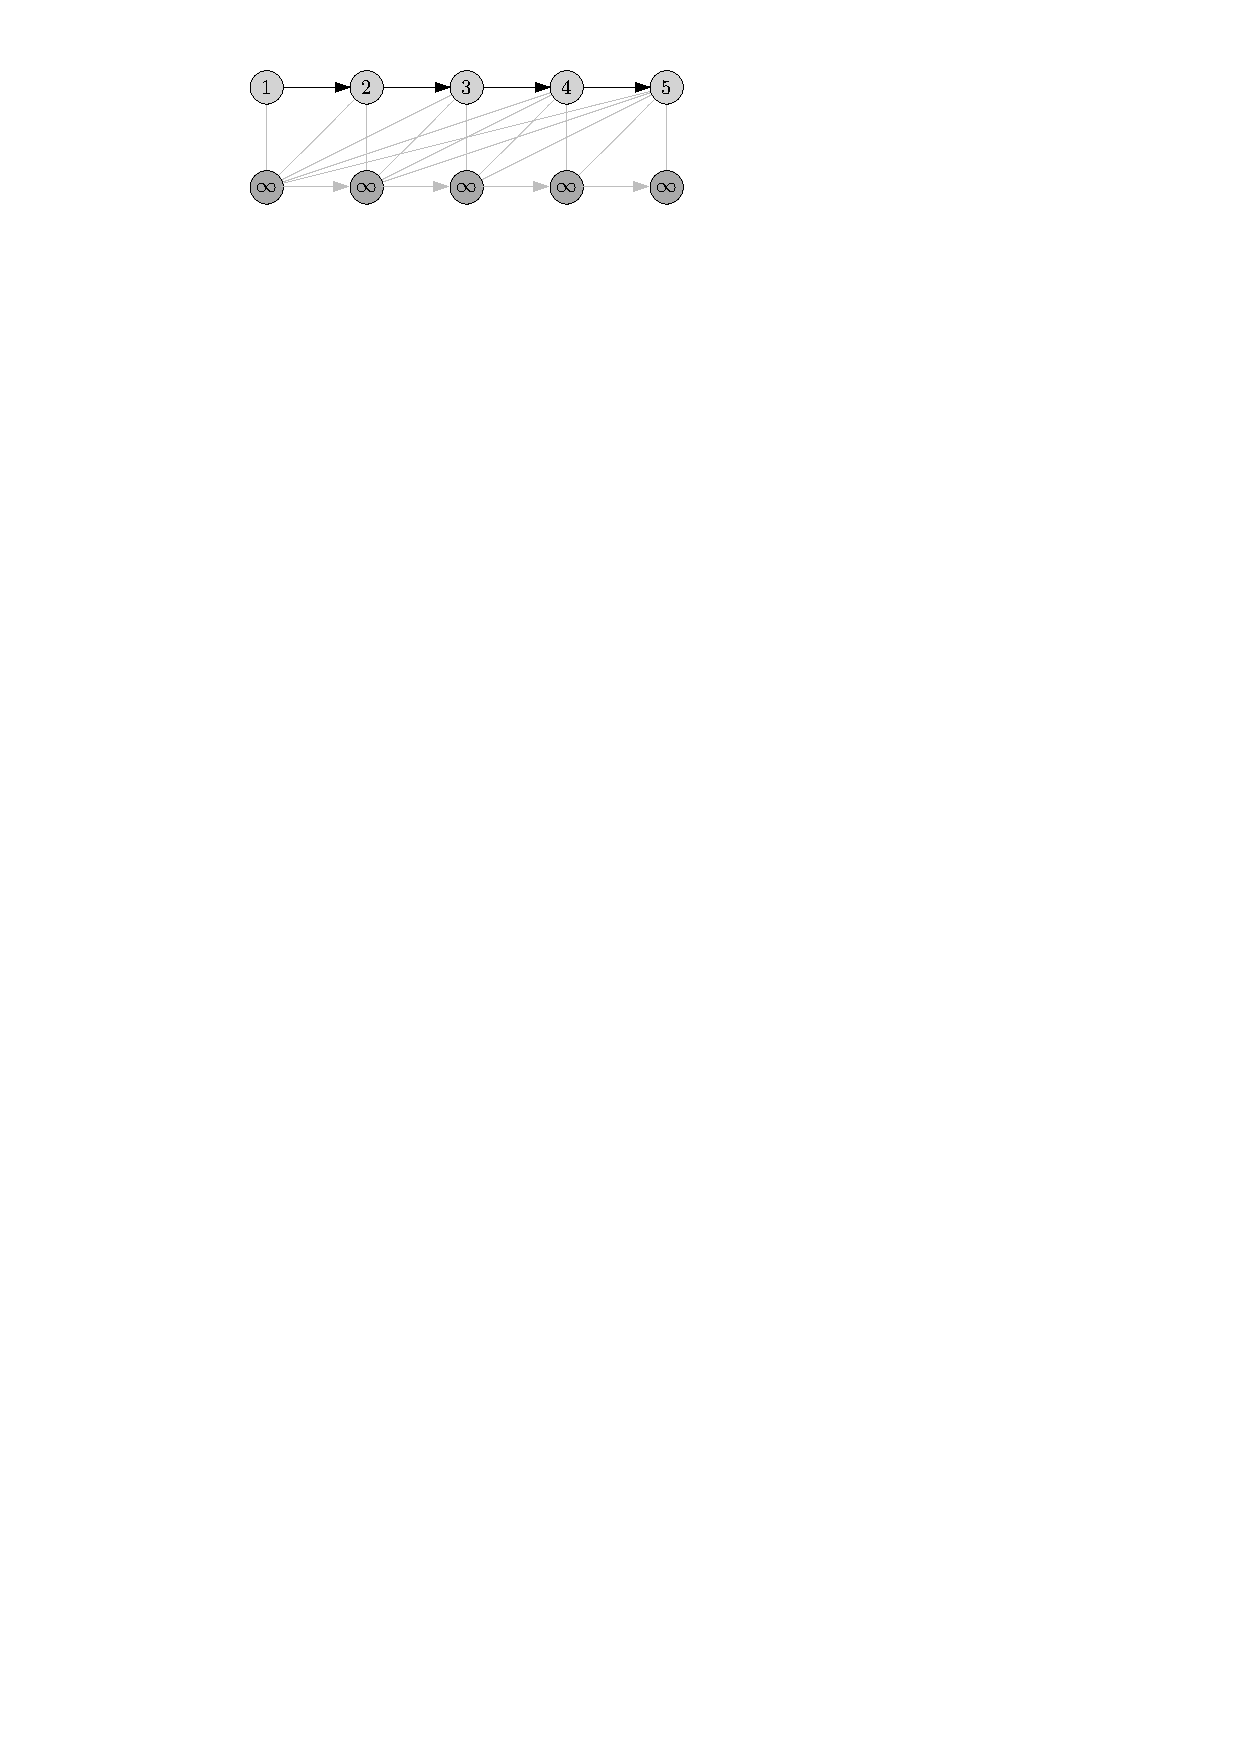
\includegraphics{figures/somegraph}
%   \caption{A funny graph.}
%   \label{fig:somegraph}
% \end{figure}

\section{Notations}
\begin{enumerate}
    \item \textbf{RLS:} Randomised local Search
    \item \textbf{(1+1) EA:} The Standard (1+1) EA
    \item \textbf{RSH:} Randomised Search Heuristics referring to all in this context analysed Evolutionary algorithms
    \item \textbf{bin:} When solving Partition a set of numbers is divided into to distinct subsets and in this paper both subsets are referred to as bins
    \item \textbf{$b_F$:} The fuller bin
    \item \textbf{$b_F$:} The emptier bin
    \item \textbf{$b_{w_i}$:} The bin containig the object $w_i$
    \item \textbf{n:} The input length of the problem
    \item \textbf{x:} A vector $x \in {\{0, 1\}}^n$ describing a solution
    \item \textbf{W:} The sum of all values $\sum_{i=1}^{n}w_i$
\end{enumerate}
\newpage

\chapter{Improving bounds on the RLS and (1+1) EA}\label{ch:Content1}

\section{Improving bounds on the RLS and the (1+1) EA}

\begin{lemma}\label{lemma:CWittRefined}
    Let $w_1\ge W/2$, then for any $\gamma$ > 1 and 0 < $\delta$ < 1, the (1+1) EA with mutation rate $c/n$ with constant $0<c<\sqrt{n}$ (\RLSR[k]) reaches an f-value at most $w_1$ + $\delta(W-w_1)$ in at most $\lceil\frac{e^c}{c\cdot(1-o(1))}n\ln(\gamma/\delta)\rceil$ $(\lceil kn\ln(\gamma/\delta)\rceil)$ steps with probability at least $1-\gamma^{-1}$. Moreover, the expected number of steps is at most $2\lceil\frac{e^c}{c\cdot(1-o(1))}n\ln(2/\delta)\rceil$ $(2\lceil kn\ln(2/\delta)\rceil)$.
\end{lemma}
\begin{proof}
    This Lemma is very similar to C. Witt's  Lemma 2 from section `2. Definitions and Proof Methods' in~\cite{witt2005worst}.
    The proof is almost the same.
    He first defines a potential function $p(x)=f(x)-l$.
    While $p(x)>0$ all steps moving only a small object to the emptier bin are accepted.
    The expected p-decrease is at least $p_0\cdot q$ where $q$ is a lower bound on the probability of the algorithm to flip one specific bit.
    This leads to a next $p$ value of $(1-q)p_0$.
    Since all steps of both algorithms are independent this argumentation remains valid even if the $p$ value is only an expected value.
    With $q=1/yn$ for a constant $y>0$ the expected $p$ value after $t=yn\ln(\gamma/\delta)$ steps is at most
    \[p_t\le p_0{(1-1/yn)}^t=p_0{(1-1/yn)}^{yn\ln(\gamma/\delta)}\le p_0\cdot e^{-\frac{1}{y}\cdot yn\ln(\gamma/\delta)}=p_0{(\gamma/\delta)}^{-1} = p_0(\delta/\gamma)\]
    Applying Markov's inequality to the non-negative $p$ value implies $p_t\le p_0\delta$ with probability $1-1/\gamma$.
    Repeating independent phases of length $\lceil yn\ln(2/\delta)\rceil$ the expected number of phases is at most 2.
    Up until here the proof is the same.\newline
    Instead of choosing $W/2$ as the general upper bound for $p_0$ as in the original lemma here the lower value $W-w_1\le W/2$ is chosen because it is more tight for the special case $w_1\ge W/2$ with $l=w_1$.
    The probability of the \RLSR[k] to flip one specific bit is \(\frac{1}{k}\cdot\frac{1}{n}\) and for (1+1) EA with mutation rate $c/n$ at least
    \[
        \frac{c}{n}{(1-\frac{c}{n})}^{n-1}
        \ge \frac{c}{n}{(1-\frac{c}{n})}^{n}
        \ge \frac{c}{n}e^{-c}(1-\frac{c^2}{n})
        = \frac{c}{e^c n}(1-o(1))
        % =\frac{c}{n}\cdot\frac{1}{1-\frac{c}{n}}{(1-\frac{c}{n})}^{n}
        % \ge\frac{c}{e^c n}\cdot(1+\frac{\frac{c}{n}}{1-\frac{c}{n}})
        % =\frac{c}{e^c n}\cdot(1+\frac{1}{\frac{n}{c}-1})
        % =\frac{c}{e^c n}\cdot(1+o(1))
    \]
    The inequality \({(1+x/n)}^n\ge e^x (1-{x^2}/n)\) requires $n\ge1, |c|\le n$ which both hold.
    Setting $y=\frac{e^c n}{c\cdot(1-o(1))}$ for the (1+1) EA and $y=k$ for the \RLSR~concludes the result.
\end{proof}

\begin{lemma}\label{lemma:W1FlipWontHappen}
    For instances with $w_1>W/2$ the probability of flipping $w_1$ when $b_E = c\cdot\frac{W-w_1}{2}$ for $1<c<2$ holds, is at most \(\frac{2y{(y-1)}^2}{n(n-1)(c-1)}\) in a step where any algorithm flips $2\le y\le n/2$ bits.
\end{lemma}
\begin{proof}
    For a successful flip of $w_1$ after $b_E \ge \frac{W-w_1}{2}$ holds a total volume of at least $z\ge2\cdot(b_E-\frac{W-w_1}{2})$ must be shifted from $b_E$ to $b_F$.
    Otherwise the step is rejected because
    \[b_F'=b_E+w_1-z>b_E+w_1-2\cdot(b_E-\frac{W-w_1}{2})=b_E+w_1-2b_E+W-w_1=W-b_E=b_F\]
    which results in an increase of the fitness ($b_F = f(x), b_F' = f(x')$).
    Let $I$ be the set of indices of all elements moved from $b_E$ to $b_F$ and $w_{\max}=\max{\{w_i|i\in I\}}$.
    $|I|\le y-1$ holds because at least $w_1$ is moved from $b_F$ to $b_E$.
    The sum of all element is at most $w_{\max} \cdot |I| \le (y-1)w_{\max}$.
    If \(w_{\max}<2\cdot(b_E-\frac{W-w_1}{2})/(y-1)\) then \((y-1)w_{\max}<2\cdot(b_E-\frac{W-w_1}{2})\) and the step is rejected.
    Thus at least one of the objects moved from $b_E$ to $b_F$ must have a volume of at least $2\cdot(b_E-\frac{W-w_1}{2})/(y-1)$.
    At most \(d\le\frac{b_E}{w_{\max}}\) of these objects can be in $b_E$ if they made up the complete volume of $b_E$. Simplifying this inequality leads to at most
    \[
        d \le \frac{b_E}{w_{\max}}
        \le \frac{W-w_1}{w_{\max}}
        \le \frac{W-w_1}{2(c\frac{W-w_1}{2}-\frac{W-w_1}{2})/(y-1)}
        = \frac{(W-w_1)(y-1)}{(W-w_1)(c-1)}
        = \frac{(y-1)}{(c-1)}
    \]
    objects having at least a volume of $w_{\max}$.
    For a successful flip $w_1$ and at least one of these $d$ objects must switch bins and the probability for such a step flipping $y$ bits is therefore at most
    \begin{gather}
        \nonumber \probP(y \text{ bits are flipped})\cdot\probP(\text{the correct $y$ bits are flipped} | y \text{ bits are flipped})\\ \nonumber
        \le 1\cdot \frac{\binom{1}{1}\cdot\binom{\lceil d\rceil}{1}\cdot\binom{n-2}{y-2}}{\binom{n}{y}}
        =\frac{\lceil d\rceil\frac{(n-2)!}{(n-2-y+2)!\cdot (y-2)!}}{\frac{n!}{(n-y)!\cdot y!}}
        =\frac{\lceil d\rceil\cdot(n-2)!\cdot(n-y)!\cdot y!}{n!\cdot(n-y)!\cdot(y-2)!}
        = \frac{\lceil d\rceil y{(y-1)}}{n(n-1)}\\ \nonumber
        \le \frac{y{(y-1)}}{n(n-1)}\cdot(\frac{y-1}{c-1}+1)
        = \frac{y{(y-1)}}{n(n-1)}\cdot(\frac{y-1+c-1}{c-1})
        \le \frac{2y{(y-1)}^2}{n(n-1)(c-1)}
    \end{gather}
\end{proof}

\begin{theorem}\label{theo:OneMaxResult}
    If $w_1 \ge \frac W 2$  then the RLS and the (1+1) EA with mutation rate $k/n$ with constant $0<k<\sqrt{n}$ reach the optimal solution in expected time $\Theta(n\log{}n)$
\end{theorem}
\begin{proof}
    The optimal solution is putting $w_1$ in one bin and all other elements in the other bin.
    So the problem is almost identical to OneMax/ZeroMax.
    A single bit flip of the first bit can only happen, if the emptier bin has a weight of at most $\frac {W-w_1}{2}$.
    After this flip the weight of the emptier bin is at least $\frac {W-w_1}{2}$ and therefore another single bit flip of $w_1$ can onl
    The run of the RLS can be divided into two phases:
    \begin{itemize}
        \item[Phase 1:] The RLS reaches a search point with $b_E > \frac {W-w_1}{2}$.
        \item[Phase 2:] The RLS reaches an optimal solution $\Rightarrow w_1$ is in one bin and all other elements are in the other bin.
    \end{itemize}

    The expected length of the first phase is at most $2n$ because the probability of flipping the first bit is $\frac{1}{n}$ and the expected time for such a step then is at most $n$.
    After such a step $b_E \ge \frac {W-w_1}{2}$ holds.
    If the solution is already optimal $b_E = W-w_1>\frac {W-w_1}{2}$, otherwise there is at least one bit that can be flipped.
    This bit will be flipped in expected time at most $n$ for the same reason as for $w_1$.
    The total length of first phase is at most $2n$.
    In the second phase the RLS can no longer flip $w_1$ as it does not result in an improvement ever again.
    Therefore the RLS behaves exactly as on OneMax/ZeroMax depending on the value of the first bit and reaches an optimal solution in $\Theta(n\log{}n)$ resulting in a total runtime of $\Theta(n\log{}n)$ (Theorem 3 in~\cite{witt2014fitness}).\newline
    As long as $w_1$ does not flip the (1+1) EA has to minimize a linear function of $n-1$ bits which takes $(1+o(1))\frac{e^k}{k}n\ln n$ time (Corollary 4.2 in~\cite{witt2013tight}).
    The only steps that could hinder the algorithm from optimising the linear function in $\Theta(n\log{}n)$ would be a flip of the first bit.
    Such steps invert the optimal solution which could decrease the progress of minimising the linear function.
    If such a step has an expected time of $\omega(n\log{}n)$ the linear function is likely to be optimised in expectation before such a step happens.
    % The probability of the (1+1) EA to flip more than $1+\sqrt{6\ln(n)}$ is limited by Chernoff bounds:
    % \begin{gather}
    %     \nonumber \probP(\text{(1+1) EA flips more than }1+\sqrt{6\ln(n)}\text{ bits})\\ \nonumber
    %     \le\probP(X\ge (1+\sqrt{6\ln(n)})\cdot 1)
    %     \le e^{-1\cdot{\sqrt{6\ln(n)}}^2/3}
    %     = e^{-6\ln(n)/3}
    %     = n^{-2}
    % \end{gather}
    % So the expected time for such a step is at least \(n^2=\omega(n\ln(n))\).
    % Now let's look at steps that flip at most $1+\sqrt{6\ln(n)}$ bits in a single step.
    % Such a step only successfully flips $w_1$ if both $w_1$ is flipped and enough total volume is shifted from $b_E$ to $b_F$.
    % Due to Lemma~\ref{lemma:CWittRefined} with $\delta=\frac{1}{n}$ (for $n>1$) the solution is at most $w_1+\delta(W-w_1)$ after expected time
    % \[
    %     2\lceil en\ln(2/\delta)\rceil
    %     =2\lceil en\ln(2/\frac{1}{n})\rceil
    %     =2\lceil en\ln(2n)\rceil
    %     =2\lceil en(\ln(n)+\ln(2))\rceil
    %     \le 2en\ln(n)+4
    % \]
    % The value of $b_E$ is then at least \(W-(w_1+\delta(W-w_1))=(1-\delta)(W-w_1)=(1-\frac{1}{n})(W-w_1)\).
    % Lemma~\ref{lemma:W1FlipWontHappen} states that the probability of a step flipping with $w_1$ together with $y-1$ other bits is at most $\frac{2y{(y-1)}^2}{n(n-1)(c-1)}$.
    % Applying the bound $y\le1+\sqrt{6\ln(n)}$ and the value $c=2(1-\frac{1}{n})$ this simplifies to
    % \[
    %     \frac{2y{(y-1)}^2}{n(n-1)(c-1)}
    %     \le\frac{2{(1+\sqrt{6\ln(n)})}^3}{n(n-1)(1-\frac{2}{n})}
    %     =\frac{2{(1+\sqrt{6\ln(n)})}^3}{n(n-1)\frac{n-2}{n}}
    %     =\frac{2{(1+\sqrt{6\ln(n)})}^3}{(n-1)(n-2)}
    % \]
    % The probability of one of these steps to happen for any value of $y$ is given by
    % \begin{gather}
    %     \nonumber \sum_{y=2}^{1+\sqrt{6\ln(n)}}{\probP(y \text{ bits are flipped})\cdot\probP(\text{the correct $y$ bits are flipped} | y \text{ bits are flipped})}\\
    %     \nonumber \le ({1+\sqrt{6\ln(n)}})\cdot\frac{2{(1+\sqrt{6\ln(n)})}^{3}}{(n-2)(n-1)}
    %     = \frac{2{(1+\sqrt{6\ln(n)})}^{4}}{(n-2)(n-1)}\\ \nonumber
    %     = \frac{2{(o({n}^{1/8}))}^{4}}{(n-2)(n-1)}
    %     = \frac{o(n^{0.5})}{\mathcal{O}(n^{2})}
    %     = \mathcal{O}(n^{-1.5})
    % \end{gather}
    % The expected time for such a step is then $\Omega(n^{1.5})=\omega(n\ln n)$.
    % The probability that such a step still happens before the linear function is optimised is at most
    % \[
    %     \frac{1}{\mathcal{O}(n^{1.5})}\cdot(1+o(1))en\ln n
    %     % =\frac{(1+o(1))en\ln n}{\mathcal{O}(n^{1.5})}
    %     =\frac{(1+o(1))e\ln n}{\mathcal{O}(n^{0.5})}
    %     =\frac{o(n^{0.1})}{\mathcal{O}(n^{0.5})}
    %     =o(\frac{1}{n^{0.4}})=o(1)\]
    % The probability of $w_1$ not being flipped after expected time $2en\ln n+4$ is \(1-o(\frac{1}{n^{0.4}})=1-o(1)\).
    % If such a step happens the fitness does not decrease and the bound on the probability of flipping $w_1$ still holds.
    % The algorithm will still find the solution in expected time at most $(1+o(1))en\ln n$.
    % Since even after a flip all condition are still true the expected time of optimising the linear function after expected time $2en\ln n+4$ is given by \(\frac{1}{1-o(1)}\cdot(1+o(1))en\ln n=\Theta(n\log{}n)\)

    % The total runtime for the (1+1) EA is $(2en\ln n+4) + \frac{1+o(1)}{1-o(1)}\cdot en\ln n =\Theta(n\log{}n)$.
    
    
    % \(\frac{1}{1-o(\frac{1}{n^{0.4}})}=\frac{1-o(\frac{1}{n^{0.4}})+o(\frac{1}{n^{0.4}})}{1-o(\frac{1}{n^{0.4}})}=1+\frac{o(\frac{1}{n^{0.4}})}{1-o(\frac{1}{n^{0.4}})}\)

    % \begin{gather}\nonumber
    %     E(T)\le\frac{E(T*)}{1-p_{\text{fail}}}
    %     \le\frac{E(T*)}{1-(E(T*)p)}
    %     =\frac{1}{\frac{1}{E(T*)}-p}
    %     =\frac{1}{\frac{1}{(1+o(1))en\ln n}-\mathcal{O}(n^{-1.5})}\\ \nonumber
    %     =\frac{1}{\frac{1-\mathcal{O}(n^{-1.5})\cdot(1+o(1))en\ln n}{(1+o(1))en\ln n}}
    %     =\frac{(1+o(1))en\ln n}{1-\mathcal{O}(n^{-1.5})\cdot(1+o(1))en\ln n}
    %     =\frac{(1+o(1))en\ln n}{1-o(\frac{1}{n^{0.4}})}
    % \end{gather}

    % So in conclusion a step moving the first bit after expected time $2en\ln n+4$ has passed is either unlikely due to the amount of bits shifted or due to the small amount of values needed to be flipped for such a step.
    % The expected time for such a step is $\omega(n\ln(n))$ and will therefore not happen in expectation before the linear function is optimised.

    % -----------------------\newline

    The probability of the (1+1) EA to flip more than $k+\sqrt{6k\ln(n)}=k+k\sqrt{6\ln(n)/k}$ is limited by Chernoff bounds:
    \begin{gather}
        \nonumber \probP(\text{(1+1) EA flips more than }k+k\sqrt{6\ln(n)/k}\text{ bits})\\ \nonumber
        \le\probP(X\ge (1+\sqrt{6\ln(n)/k})\cdot k)
        \le e^{-k\cdot{\sqrt{6\ln(n)/k}}^2/3}
        = e^{-k\cdot \frac{6\ln n}{3k}}
        = n^{-2}
    \end{gather}
    So the expected time for such a step is at least \(n^2=\omega(n\ln(n))\).
    Now let's look at steps that flip at most $k+\sqrt{6k\ln(n)}$ bits in a single step.
    Such a step only successfully flips $w_1$ if both $w_1$ is flipped and enough total volume is shifted from $b_E$ to $b_F$.
    Due to Lemma~\ref{lemma:CWittRefined} with $\delta=\frac{1}{n}$ (for $n>1$) the solution is at most $w_1+\delta(W-w_1)$ after expected time
    \begin{gather}\nonumber
        2\lceil\frac{e^k}{k(1-o(1))}n\ln(2/\delta)\rceil
        =2\lceil\frac{e^k}{k(1-o(1))}n\ln(2/\frac{1}{n})\rceil
        =2\lceil\frac{e^k}{k(1-o(1))}n\ln(2n)\rceil \\ \nonumber
        =2\lceil\frac{e^k}{k(1-o(1))}n(\ln(n)+\ln(2))\rceil
        \le\frac{2e^k}{k(1-o(1))}n\ln(n)+4
    \end{gather}
    The value of $b_E$ is then at least \(W-(w_1+\delta(W-w_1))=(1-\delta)(W-w_1)=(1-\frac{1}{n})(W-w_1)\).

    Lemma~\ref{lemma:W1FlipWontHappen} states that the probability of a step flipping with $w_1$ together with $y-1$ other bits is at most $\frac{2y{(y-1)}^2}{n(n-1)(c-1)}$.
    Applying the bound $y\le k+\sqrt{6k\ln(n)}$ and the value $c=2(1-\frac{1}{n})$ this simplifies to
    \[
        \frac{2y{(y-1)}^2}{n(n-1)(c-1)}
        \le\frac{2{(k+\sqrt{6k\ln(n)})}^3}{n(n-1)(1-\frac{2}{n})}
        =\frac{2{(k+\sqrt{6k\ln(n)})}^3}{n(n-1)\frac{n-2}{n}}
        =\frac{2{(k+\sqrt{6k\ln(n)})}^3}{(n-1)(n-2)}
    \]
    The probability of one of these steps to happen for any value of $y$ is given by
    \begin{gather}
        \nonumber \sum_{y=2}^{k+\sqrt{6k\ln(n)}}{\probP(y \text{ bits are flipped})\cdot\probP(\text{the correct $y$ bits are flipped} | y \text{ bits are flipped})}\\
        \nonumber \le ({k+\sqrt{6k\ln(n)}})\cdot\frac{2{(k+\sqrt{6k\ln(n)})}^{3}}{(n-2)(n-1)}
        = \frac{2{(k+\sqrt{6k\ln(n)})}^{4}}{(n-2)(n-1)}\\ \nonumber
        = \frac{2{(o({n}^{1/8}))}^{4}}{(n-2)(n-1)}
        = \frac{o(n^{0.5})}{\mathcal{O}(n^{2})}
        = \mathcal{O}(n^{-1.5})
    \end{gather}

    The expected time for any step successfully flipping $w_1$ is then $\Omega(n^{1.5})=\omega(n\ln n)$.
    Let $T$ be the time until the linear function is optimised and $p$ the probability of successfully flipping $w_1$.
    Then the probability that $w_1$ flips after expected time $\frac{2e^k}{k(1-o(1))}n\ln(n)+4$ before the linear function is optimised is at most
    \[
        p\cdot E(T) \le \frac{1}{\mathcal{O}(n^{1.5})}\cdot(1+o(1))\frac{e^k}{k}n\ln n
        % =\frac{(1+o(1))\frac{e^k}{k}n\ln n}{\mathcal{O}(n^{1.5})}
        =\frac{(1+o(1))\frac{e^k}{k}\ln n}{\mathcal{O}(n^{0.5})}
        =\frac{o(n^{0.1})}{\mathcal{O}(n^{0.5})}
        =o(\frac{1}{n^{0.4}})=o(1)\]
    The probability of $w_1$ not being flipped after expected time $\frac{2e^k}{k(1-o(1))}n\ln(n)+4$ is \(1-o(\frac{1}{n^{0.4}})=1-o(1)\).
    If such a step happens the fitness does not decrease and the bound on the probability of flipping $w_1$ still holds.
    The algorithm will still find the solution in expected time at most $(1+o(1))\frac{e^k}{k}n\ln n$.
    Since even after a flip all condition are still true the expected time of optimising the linear function after expected time $\frac{2e^k}{k(1-o(1))}n\ln(n)+4$ is given by \(\frac{1}{1-o(1)}\cdot(1+o(1))\frac{e^k}{k}n\ln n=\Theta(n\log{}n)\)

    The total runtime for the (1+1) EA is $\frac{2e^k}{k(1-o(1))}n\ln(n)+4 + \frac{1+o(1)}{1-o(1)}\cdot \frac{e^k}{k}n\ln n =\Theta(n\log{}n)$.

\end{proof}

\begin{lemma}\label{approximationLemmaHelp1}
    If \(b_F \le \frac{2}{3} \cdot W\) the approximation ratio is at most $\frac{4}{3}$
\end{lemma}
\begin{proof}
    \(\frac{b_F}{opt} \le \frac{(2/3) \cdot W}{opt} \le \frac{(2/3) \cdot W}{(1/2) \cdot W} = \frac{4}{3}\), since \(opt \ge \frac{W}{2}\)
\end{proof}

\begin{corollary}\label{approximationCorollaryHelp2}
    If \(w_1 \ge \frac{W}{3}\) and \(w_1\) is in the emptier bin, then the approximation ratio is at most $\frac{4}{3}$
\end{corollary}
\begin{proof}
    $w_1$ is in the emptier bin, so \( b_F \le W - w_1 \le W - \frac{W}{3} = \frac{2W}{3} \) and with Lemma~\ref{approximationLemmaHelp1} the assumption follows.
\end{proof}

\begin{lemma}\label{movingObjectsLemma}
    Any object of weight $v$ can be moved from $b_F$ to $b_E$ if and only if \(b_F - b_E \ge v\)
\end{lemma}
\begin{proof}
    $''\Leftarrow''$:\newline
    \(b_F - b_E \ge v \Leftrightarrow b_F \ge b_E + v\), so after moving an object with weight $v$ from $b_F$ to $b_E$, the new weight of $b_E$ is at most the weight of $b_F$ before moving the object, thus the RSH accepts the step.\newline
    $''\Rightarrow''$:\newline
    \(b_F - b_E < v \Leftrightarrow b_F < b_E + v\), so moving an object of weight $v$ results in ${b_F}' = b_E+v > b_F$ which results in the step being rejected.
\end{proof}

\begin{corollary}\label{cor:RLSStuck}
    The RLS is stuck in a local optimum if \(b_F-b_E \le w_n\) holds and \(b_F > opt\).
\end{corollary}
\begin{proof}
    A single bit flip of weight $v$ can only happen if \(b_F - b_E \ge v\) (Corollary~\ref{cor:RLSStuck}). If \(b_F-b_E < w_n\) there is no weight which satisfies the condition and therefore no single bit flip is possible.
    If \(b_F-b_E = w_n\) then only objects with weight \(w_n\) can be flipped, but those do not change the fitness ($b_F' = b_E + w_n = b_F - w_n +w_n = b_F$).
    Since the RLS can only move one bit at a time and only if it results in an improvement, the RLS is stuck.
\end{proof}

\begin{corollary}\label{movingObjectsCorollary}
    Every object \(\le \frac{W}{3}\) can be moved from $b_F$ to $b_E$ if \(b_F \ge \frac{2W}{3}\)
\end{corollary}
\begin{proof}
    \(b_F \ge \frac{2W}{3} \Rightarrow b_E \le W - \frac{2W}{3} \le \frac{W}{3} \Rightarrow b_F - b_E \ge \frac{2W}{3} - \frac{W}{3} = \frac{W}{3}\) and with Lemma~\ref{movingObjectsLemma} the assumption follows.
\end{proof}

\begin{lemma}\label{movingObjectsLemma2}
    In expected time $\mathcal{O}(n\log{}n)$ the weight of the fuller bin can be decreased to \(\le \frac{2W}{3}\) by the RLS and the (1+1) EA if every object besides the biggest in the fuller bin is at most $\frac{W}{3}$ and \(w_1 \le \frac{W}{2}\).
\end{lemma}
\begin{proof}
    In expected time $\mathcal{O}(n\log{}n)$ the RSH can move every object $\le \frac{W}{3}$ to the emptier bin as long as $b_F \ge \frac{2W}{3}$ due to Corollary~\ref{movingObjectsCorollary} and Theorem~\ref{theo:OneMaxResult}.
    So in expected time $\mathcal{O}(n\log{}n)$ the solution can be shifted to $w_1$ being in one bin and all other objects in the other bin.
    The RSH will only stop moving the elements if the condition $b_F \ge \frac{2W}{3}$ is no longer satisfied (Corollary~\ref{movingObjectsCorollary}).
    If \(w_1 \ge \frac{W}{3}\) and every object was moved to the bin without $w_1$, then \(b_F = \max\{W-w_1, w_1\} = W-w_1 \le \frac{2W}{3}\), because \(w_1 \le \frac{W}{2}\).
    So either the RSH moves all objects to the emptier bin or stops moving objects because $b_F < \frac{2W}{3}$ both resulting in $b_F \le \frac{2W}{3}$.
    If $w_1$ is not in the fuller bin, then the result follows by Corollary~\ref{approximationCorollaryHelp2}.\newline
    Now assume \(w_1 < \frac{W}{3}\).
    In this case the RLS will move one object per step to the emptier bin.
    Each object has weight $< \frac{W}{3}$ and therefore one step cannot decrease the weight of the fuller bin from $> \frac{2W}{3}$ to $\le \frac{W}{3}$.
    If all objects except one where moved to one bin, the other bin would have a weight of at least \(W-w_1 > \frac{2W}{3}\).
    Therefore the RLS will find a solution with $b_F < \frac{2W}{3}$ before moving all elements from the first to the second bin.\newline
    The proof for the (1+1) EA is mostly the same.
    The main difference is the (1+1) EA being able to flip more than one bit in a single step.
    Such a step could make the emptier bin the fuller bin or increase the number of bits that must be shifted to the emptier bin.
    But with the results of Theorem~\ref{theo:OneMaxResult} the proof works exactly the same as for the RLS.\
    The case \(w_1 \ge \frac{W}{3}\) does not change only the bin containing $w_1$ might change.
    Apart from that there is no difference for the (1+1) EA.\
    The case $w_1 < \frac{W}{3}$ is also rather similar.
    The (1+1) EA will move elements from the fuller bin to the emptier bin until $b_F < \frac{2W}{3}$ holds. The (1+1) EA can make the emptier bin the fuller bin by moving multiple objects in one step, but this does not hinder it from reaching $b_F < \frac{2W}{3}$. After such a step it will continue moving elements until the condition holds.
\end{proof}

\begin{lemma}\label{approximationLemma}
    The RLS and the (1+1) EA reach an approximation ratio of at most $\frac{4}{3}$ in expected time $\mathcal{O}(n\log{}n)$ if $w_1 < W/2$
\end{lemma}
\begin{proof}
    If \(w_1+w_2 > \frac{2W}{3}\) after time $\mathcal{O}(n)$ $w_1$ and $w_2$ are separated and will remain separated afterwards (3. Average case analysis, Theorem 1 in~\cite{witt2005worst}).
    From then on the following holds.
    If $w_1$ is in the emptier bin, then the result follows directly by Corollary~\ref{approximationCorollaryHelp2}.
    Otherwise all elements in the fuller bin except $w_1$ have a weight of at most $\frac{1}{3}$ and therefore the result follows by Lemma~\ref{movingObjectsLemma2} and Lemma~\ref{approximationLemmaHelp1}.
    If \(w_1+w_2 \le \frac{2W}{3}\) the result follows directly by Lemma~\ref{movingObjectsLemma2} and Lemma~\ref{approximationLemmaHelp1}.
\end{proof}

\begin{corollary}
    The RLS and the (1+1) EA reach an approximation ratio of at most $\frac{4}{3}$ for every input in expected time $\mathcal{O}(n\log{}n)$
\end{corollary}
\begin{proof}
    This follows directly from Theorem~\ref{theo:OneMaxResult} and Lemma~\ref{approximationLemma}.
\end{proof}

\section{Binomial distributed input}
\begin{lemma}\label{lemma:BinomialSolvable}
    A binomial distributed input \textasciitilde$B(m,p)$ has a perfect partition ($b_F - b_E = 0$ for even $W$ and $b_F - b_E = 1$ for uneven $W$) with high probability if the input size $n$ is large enough.
\end{lemma}
\begin{proof}
    Sketch:
    \begin{itemize}
        \item The initial distribution is likely rather close to the optimum
        \item The difference between the bins is probably not more than 10 expected values
        \item the large values
    \end{itemize}
    Consider a random separation of all values into two sets with equal size if $n$ is even or one set with one value more than the other if $n$ is odd. The sum X of one set is a sum of $\frac{n}{2}\cdot m$ independent Bernoulli trials with probability $p$. With Chernoff Bounds the following inequality follows:
    \[\probP(X\ge(\frac{n}{2}+\sqrt{\frac{n}{2}})\cdot m \cdot p) = \probP(X\ge(1+2\sqrt{\frac{2}{n}})\cdot \frac{nmp}{2}) \le e^{-\frac{mnp}{2}\cdot2\sqrt{\frac{2}{n}}^2 /3} = e^{-\frac{2mp}{3}}\]
    For $mp\ge1.5$ the probability is less than $\frac{1}{e}$. Otherwise the input is rather trivial, since the numbers will be concentrated around $mp\le1.5$ and most values will be below 10.\newline
    After moving $\mathcal{O}(\sqrt{\frac{n}{2}}/2)$ objects to the emptier set, the difference between the two sets is at most half the expected value $mp$ of a single value.
    \dots
\end{proof}


\begin{lemma}
    With high probability the RLS does not find an optimal solution for an input with distribution \textasciitilde$B(m,p)$ if n and m are large enough.
\end{lemma}
\begin{proof}
    Sketch:
    \begin{itemize}
        \item There exists an optimal solution with high probability due to last lemma
        \item probability for a value to be very low is almost 0 if m is huge
        \item The RLS only moves one element per step and will reach $b_F$-$b_E$ < $w_n$ without $b_F= opt$ being true
        \item → RLS can't make another step and is stuck in a local optimum.
    \end{itemize}
    Due to Lemma~\ref{lemma:BinomialSolvable} the input has an optimal solution with high probability. The probability for small values \dots\newline
    % As long as $b_F-b_E>w_1$ holds moving any object $w_i$ from $b_F$ to $b_E$ results in a decrease of the fitness of $w_i$.
    % The RLS will continue moving elements to the emptier bin at least until $b_F-b_E$ holds which will eventually happen because there is always at least one bit left in $b_F$ that can be shifted to the emptier bin as long as $b_F-b_E>w_1$.
    % When the RLS reaches a search point of $b_F-b_E\le w_1$ there are two cases.
    % In the first case $b_F-b_E<w_n$ which means that the RLS is stuck due to Corollary~\ref{cor:RLSStuck}.
    % In the other case $b_F-b_E\ge w_n$ holds and therefore there is at least one object left in the fuller bin, that can be moved to the emptier bin.
    % If the moved object $w_i\le (b_F-b_E/2)$ then $b_F'-b_E'=(b_F-w_i)-(b_E-w_i)\le w_1-w_n$.
    % If the moved object $w_i> b_F-b_E$ then $b_F'-b_E'=(b_F-w_i)-(b_E-w_i)=b_F-b_E-2w_i\le \dots$.

    The RLS will always move one object per step from fuller to the emptier bin.
    As long as $b_F-b_E>w_i$ holds moving any object of weight at most $w_i$ from $b_F$ to $b_E$ results in a decrease of the fitness ($b_F'=b_E+w_i<b_F-w_i+w_i=b_F$).
    If the RLS does not decrease the difference $b_F-b_E$ to at most $w_n$ the solution is never optimal and the RLS therefore must be stuck.
    So now assume the RLS eventually reaches a search point with $b_F-b_E\le w_n$.
    Consider the step wich decreases the difference from more than $w_n$ to at most $w_n$.
    If this step does not decrease the difference to 0 for even $n$ or 1 for odd $n$ the RLS is stuck due to Corollary~\ref{cor:RLSStuck}.
    For a step to decrease $b_F-b_E$ from more than $w_n$ to 0 the RLS must move an object of weight $y$ which is given by $b_F'-b_E'=(b_F-y)-(b_E+y)=0\Leftrightarrow b_F-b_E-2y=0\Leftrightarrow y=(b_F-b_E)/2$.
    Such an element can only exist for even $n$ because only for even n either both bins have an even sum or neither of them.
    Odd inputs will always have exactly one bin with an even sum and one with an odd sum.
    For odd $n$ a difference of 1 suffices for an optimal solution and therefore the value of $y$ must be either $\lceil(b_F-b_E)/2\rceil$ or $\lfloor(b_F-b_E)/2\rfloor$.
    For any binomial distribution the value which occurs the most in expectation is the expected value if $mp\in\N$ or $\lceil mp\rceil$ and $\lfloor mp\rfloor$ otherwise.
    Let's assume that exactly objects with this volume must be selected and that there are two options because $mp\notin\N$.
    This will give an upper bound on the probability of flipping the right object in the crucial step.
    The probability of a number to be $\lfloor mp\rfloor$ is $p^{\lfloor mp\rfloor}{(1-p)}^{m-\lfloor mp\rfloor}\le0.5^{50}\le\frac{1}{1024^5}\le10^{-15}$ because both $mp\ge50$ and $m-mp\ge50$ and $p\le0.5$ or $1-p\le0.5$.
    For $\lceil mp\rceil$ the same bound applies with the same arguments.
    The probability of either of these numbers to be drawn from the binomial distribution is at most $2\cdot 0.5^{50}=0.5^{49}\le10^{-15}$.
    This leads to $n\cdot 10^{-15}$ values with the right value.
    All bits are flipped uniformly at random and therefore the probability of flipping a good bit is at most \(\frac{n\cdot 10^{-15}}{n}=10^{-15}\).
    This means the RLS is very unlikely to find a perfect partition.
    Given the solution has a perfect partition the RLS will get stuck in a local optimum.

    Note: The restriction of $mp\ge50$ and $m-mp\ge50$ was not chosen to make the proof work but is also necessary.
    If the algorithm produces many small values and especially elements close to 1.
    When there are many small values these can be used to fill the small gaps which makes it easy for the RLS to find a perfect partition.
    On the other hand if $p$ is almost one, then almost every element will be same for smaller values of $m$.
    If every element is the same then the RLS must only find a search point with equal amounts of 0s and 1s.
\end{proof}